\documentclass[12pt,a4paper]{article}
\usepackage[marginparsep=8pt,left=2.5cm,right=2.5cm,top=2.5cm,bottom=3cm]{geometry}
\usepackage{graphicx}
\usepackage[czech]{babel}
\usepackage[utf8]{inputenc}
\usepackage{amsmath}
\usepackage[dvipsnames]{xcolor}
%\setlength{\parindent}{0pt}% Remove paragraph indent
\graphicspath{ {./images/} }
\newcommand*\rfrac[2]{{}^{#1}\!/_{#2}}

\newcommand{\overbar}[1]{\mkern 2.5mu\overline{\mkern-2.5mu#1\mkern-2.5mu}\mkern 2.5mu}

\usepackage[explicit]{titlesec}
\titleformat{\section}{\bf\Large}{#1}{1em}{}
\titleformat{\subsection}{\bf\large}{#1}{1em}{}

\pagenumbering{gobble} % da pryc cislo stranky na uvodni strance..

\usepackage{listings}
\lstset{
  language=Python,
  keywordstyle=\ttfamily\color{MidnightBlue},
  emph={MyClass,__init__},
  emphstyle=\ttfamily\color{Mahogany},  
  stringstyle=\color{OliveGreen},
  basicstyle=\ttfamily,
  columns=fullflexible,
  breaklines=true,
  breakatwhitespace=true,
  postbreak=\mbox{\textcolor{red}{$\hookrightarrow$}\space},
  frame=tb,
  tabsize=2,
  commentstyle=\color{Gray},      
}

%% ZAHLAVI A ZAPATI
\usepackage{fancyhdr}
\pagestyle{fancy}
\renewcommand{\sectionmark}[1]{\markright{#1}}

% prostredni cast zapati
\cfoot{\thepage}

% leva cast zahlavi -- nazev sekce/subsekce
\lhead{\fancyplain{}{\rightmark}}

% prava cast zahlavi -- logo fitu

%\rhead{
\includegraphics[width=4cm]{logo}}

%% PROKLIKAVATELNE ODKAZY -- nastaveni xetex/pdftex
\usepackage[pdftex,pdfpagelabels,bookmarks,hyperindex,hyperfigures]{hyperref}

\hypersetup{
  colorlinks,
  citecolor=blue,
  filecolor=blue,
  linkcolor=blue,
  urlcolor=blue
}

\begin{document}

\begin{titlepage}
  % pro zobrazeni loga v zahlavi
  \thispagestyle{fancy}

  % vertikalni zarovnani
  \vspace*{\fill}
  \begin{center}
    {\fontsize{20}{30}\selectfont CZ4015}\\[1cm]
    {\fontsize{30}{100}\selectfont \textbf{Final Report}}\\[4.2cm]
  \end{center}

  % vertikalni zarovnani
  \vspace*{\fill}

  % seznam clenu tymu razeny abecedne podle krestniho jmena
  {\fontsize{10}{10} \selectfont \noindent
  \textbf{Author:}\\
  Pavel Jahoda (N1800740K)
  }
\end{titlepage}

%%%%% 
\renewcommand{\headrulewidth}{0.4pt}
\renewcommand{\footrulewidth}{0.4pt}

% rimska cisla pro cislovani stranek v obsahu
\pagenumbering{roman}

% samotne vlozeni obsahu
\tableofcontents

\newpage

% zapnout bezne cislovani stranek pomoci arabskych cislic
\pagenumbering{arabic}

\section{Input Analysis}
\subsection{Cleaning data}
First we need to clean our data from mistakes made during data gathering. To do so, we will visualize our data using scatter plot. The scatter plot below visualizes how long each call lasted and how fast was the person driving when making the call.
\begin{center}
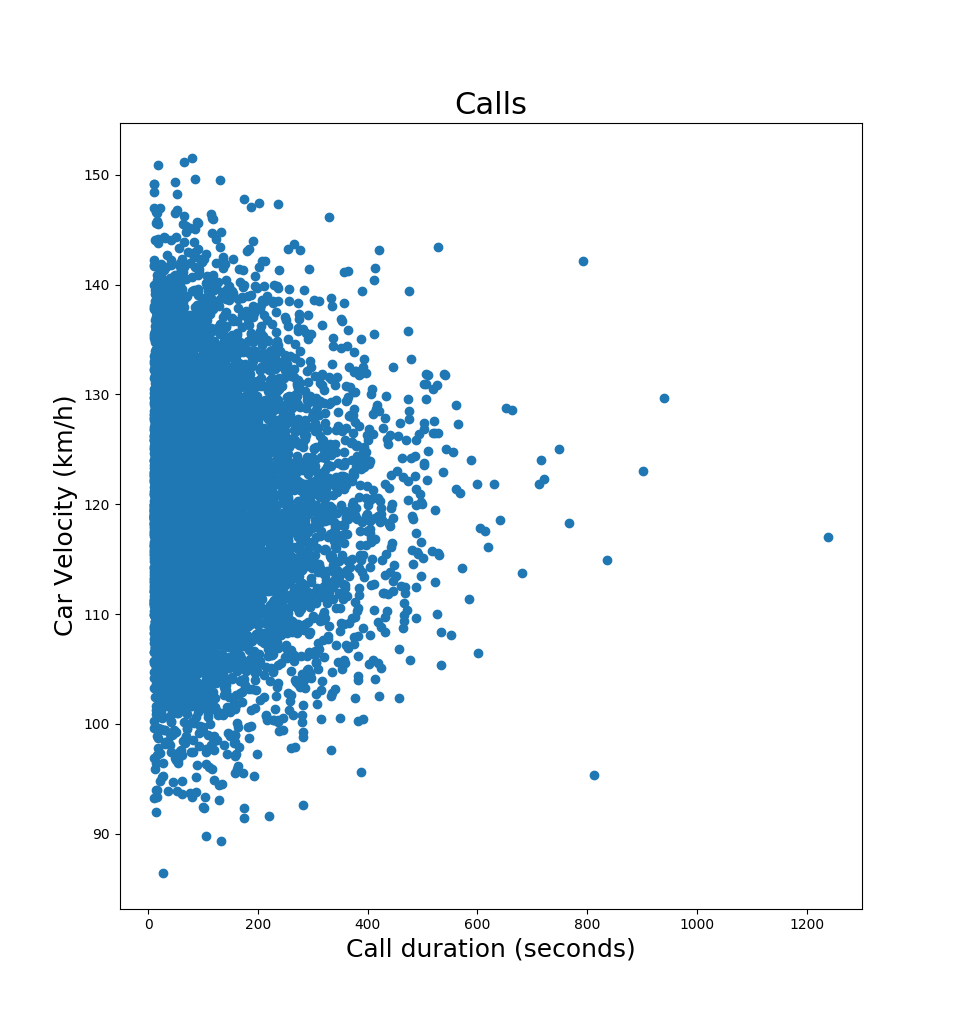
\includegraphics[width=6.5in]{Figure_0}
\end{center}
The most extreme value we can see is from a call that lasted more than 20 minutes, which is entirely possibly, so we won't delete any values. It was also checked that each call started from station between 1-20.
\pagebreak

\subsection{Distribution identification}
From the histograms below we can see similary between the distributions of inter-arrival times and call durations. Both of these histograms resemble probability density function of exponential distribution.\par
%\begin{lstlisting}
%from statsmodels.distributions.empirical_distribution import ECDF
%ecdf = ECDF(weightsSurvived)
%\end{lstlisting}
\smallskip
\noindent 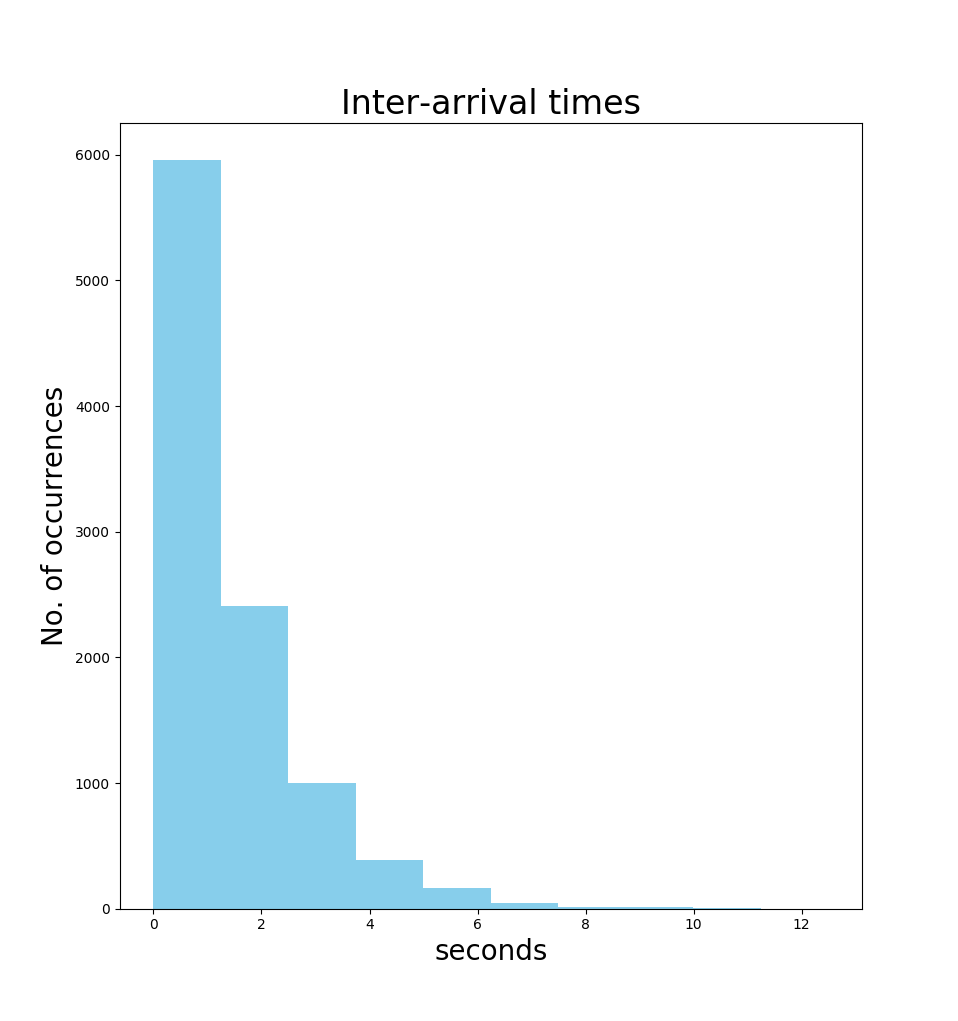
\includegraphics[width=3.4in]{Figure_1}
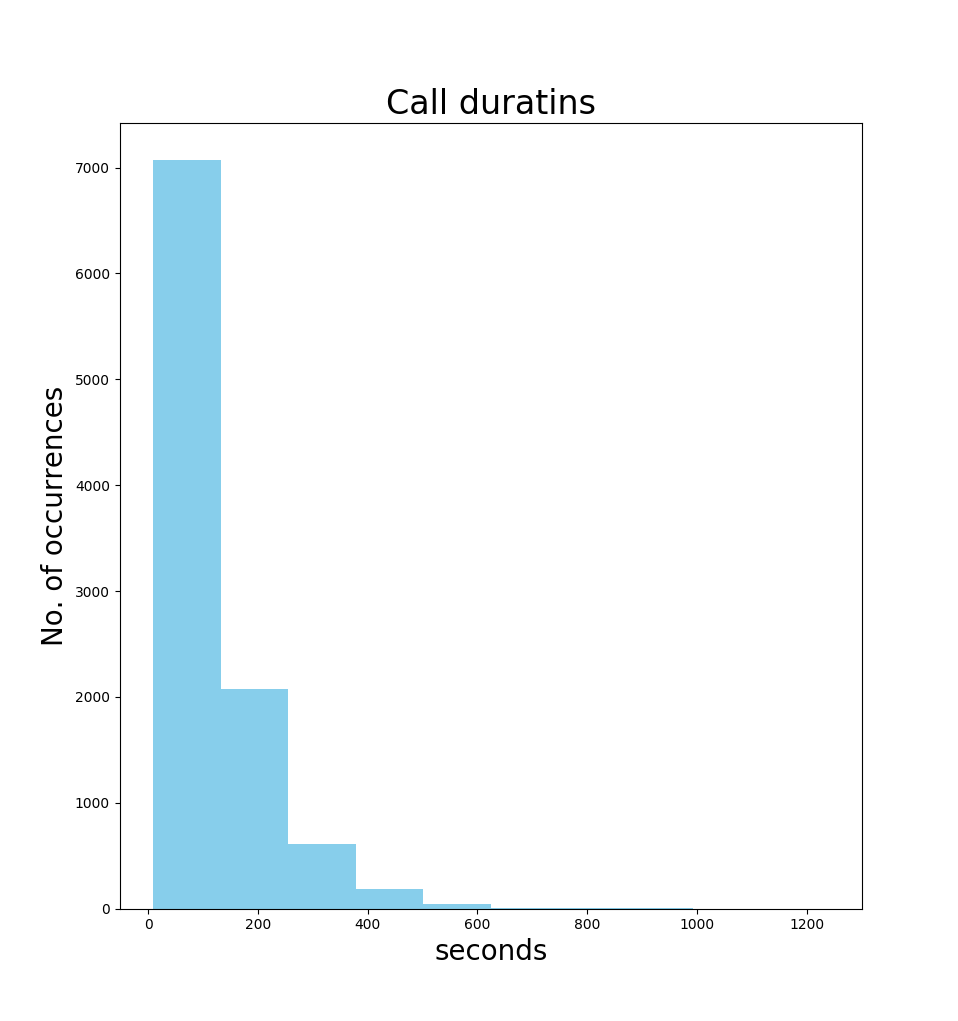
\includegraphics[width=3.4in]{Figure_3}
First, we will estimate the parameter of the exponential functions using maximum likelihood estimation.
The exponential function is denoted as:
\begin{equation} \lambda\cdot\mathrm{e}^{-\lambda\cdot x} \end{equation}
The likelihood function for the parameter lambda given $x_1$, $x_2$,..,$x_n$ is denoted as:
\begin{equation} \mathcal{L}(\lambda|x_1, x_2,..,x_n) = \lambda^{n}\cdot\mathrm{e}^{-\lambda\cdot \sum_{i=1}^{n} x_i} \end{equation}
To find the lambda for which the likelihood function is maximal, we differentiate by lambda and solve for lambda when the derivate is equal to 0, which results in the following formula:
\begin{equation} \lambda=\dfrac{n}{\sum_{i=1}^{n} x_i} \end{equation}
Using maximum likelihood function of an exponential distribution we have calculated lambda for the inter-arrival times to be $0.73$ and lambda for the call duration times to be $0.009$.

\pagebreak
On the other hand, the two histograms below show two different distributions. The histogram on the left shows that the stations where the cars are located when the call begins are uniformly distributed from 1 to 20. The histogram of the car velocities (on the right) resembles normal distribution.\par
\noindent 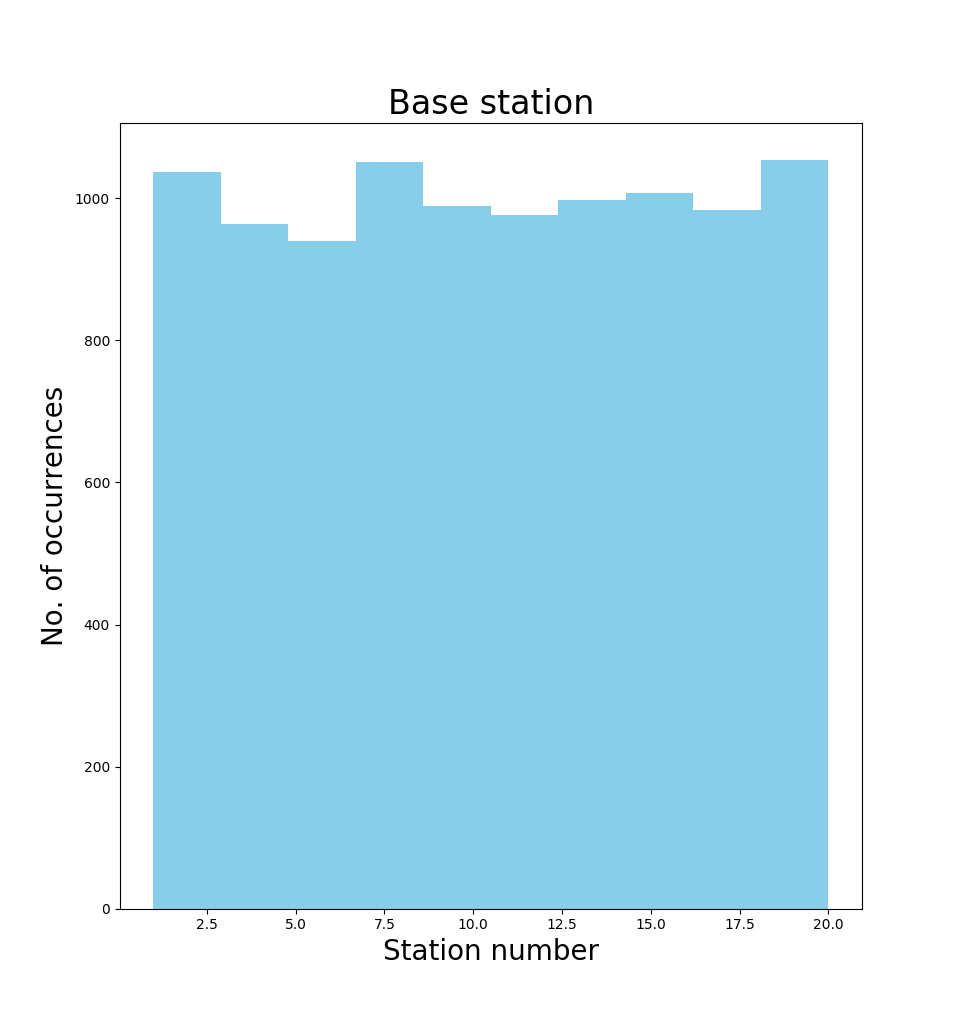
\includegraphics[width=3.4in]{Figure_2}
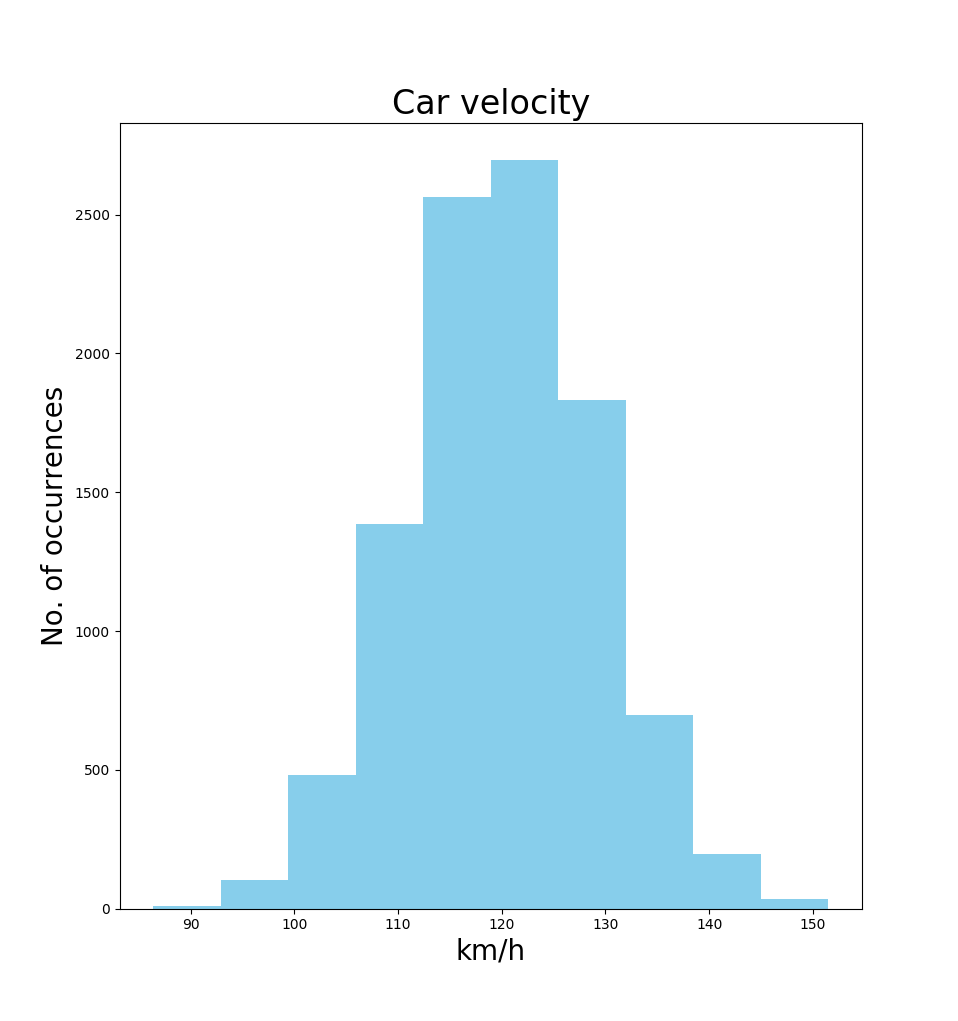
\includegraphics[width=3.4in]{Figure_4}
Similarly as with the exponential distributions above, we will use maximum likelihood method to calculate the parameters of the normal distribution (car velocities). We get $\mu=120.07$ and $\sigma^2=81.33$.

\subsection{Hypothesis Testing}
After we made distribution identification hypotheses, it is time to do hyptohesis testing. First, let's focus on testing our hypothesis about inter-arrivel times having exponential distribution with $\lambda=0.73$ using Pearson's chi-squared test, which has the following formula.
\begin{equation} {\chi}^2=\sum_{i=1}^{k} \frac{(O_i - E_i)^2}{E_i}\ \end{equation}

First we will divide the observations into $k$ mutually exclusive classes that all have the same probability that an observation falls into said class. In the formula above $E_i$ the expected value of observation's that fall into a $ith$ class and $O_i$ is the number of observed values that actually fall into $ith$ class. We define our class as an interval from $r_{i-1}$ to $r_i$ by solving the following formula.

\begin{equation} \int_{0}^{r_i}\lambda\cdot\mathrm{e}^{-\lambda\cdot x}dx = \frac{i}{k} \end{equation}
For i = 1,2,…,k. By integrating probability density function we get cumulative distribution function.
\begin{equation} 1 - \mathrm{e}^{-\lambda\cdot r_i} = \frac{i}{k} \end{equation}
Solving it for $r_i$, we get
\begin{equation} r_i = \frac{\ln(-\frac{i}{k} + 1)}{-\lambda} \end{equation}

Now that we have our classes we can compare the number of observed values in a class compared to expected number of values in the class to get our $\chi^2$ value. For the inter-arrival times, we got $\chi^2=110.53$, which is less than $\chi^2_{99, 0.05}$, so we cannot reject our null hypothesis that the inter-arrival time has an exponential distribution with $\lambda=0.73$. If the result of our chi-square test was higher than $\chi^2_{0.05}$, we could reject our null hypothesis and be $95\%$ sure our rejection was correct.
\par \medskip
Then, we perfomed chi-squared test for our other hypotheses. When performing chi-squared test for a hypothesis that call duration times have exponential distribution we got very high $\chi^2$ value, which meant we should reject our hypothesis, but after shifting the values by their lowest value the hypothesis could not have been rejected.

\section{Pseudocode}
In my first submission of the simulation pseudocode, I have made two mistakes. The first mistake was blocking the main thread while waiting for another event to happen. The issue was resolved by updating the system clock time to the time of the next event (call initiation, handover or termination). Another issue with my previous version of the pseucode was that it wasn't detailed enough to show the full functionality of the simulation system. After the issues were resolved, here is how the pseudocode looks like.
\begin{lstlisting}
# The driving and calling object
class Object(): #TODO
    def __init__(self, duration, speed, station, position, direction):
        self.duration = duration
        self.speed = speed
        self.station = station
        self.position = position
        self.direction = direction


class Simualation():
    def __init__(self):
        # system clock, which will be updated outside of events
        self.clock = 0 

        self.n_of_dropped_calls = 0
        self.n_of_blocked_calls = 0
        self.n_of_calls = 0
        self.n_of_channels_reverved = 0

        # we will update this number until we reach our 
        # desired number of initiation calls
        self.n_of_calls_created = 0 

        self.generator = Generator()

        # we will have a list-like data structure that will 
        # keep events sorted by the simulated time
        # [time of next event in seconds, type of event, 
        # Object(speed, call duration etc)]
        # type of event -> 0: i
        self.eventList = []

        # how many free channels each station currently has
        self.free_channels_by_station = [10 for i in range(20)] 

    # parameter - number of channels reserved for handovers 
    # when other channels are not available
    def simulate(self, n_of_channels_reverved):
        self.n_of_channels_reverved = n_of_channels_reverved
        
        # generate first initiation
        self.eventList.append(self.generator.generate_next_initiation()) 
        self.n_of_calls_created += 1

        while len(self.eventList) != 0:
            # update the system clock time to the time of next event
            self.clock = self.eventList[0][0]

            # depending on the type of the object in the event list, 
            # call function initiation, termination or handover
            if self.eventList[0][1] == 0: # if the event is new call, generate another call
                self.eventList.append(self.generator.generate_next_initiation())
                self.initiation()
            elif self.eventList[0][1] == 1: # handover
                self.handover()
            else: # termination
                self.termination()

            # after we make the call we update the event list and remove the first item
            self.eventList = self.eventList[1:]
            self.eventList.sort()
            
            if self.n_of_calls_created == 10000: #some desired number of calls
                break

        return self.n_of_blocked_calls, self.n_of_dropped_calls, self.n_of_calls, self.n_of_channels_reverved

    def CalculateHowLongTillNextEvent(self,position, speed, direction):
        kmTillNextEvent = position % 2  # position modulo 2
        kmTillNextEvent = kmTillNextEvent + 2 if kmTillNextEvent == 0 else kmTillNextEvent

        if direction == 'RIGHT' and kmTillNextEvent != 2:
            kmTillNextEvent = 2 - kmTillNextEvent

        return kmTillNextEvent/speed * 3600 # in seconds

    def initiation(self, obj):
        if self.free_channels_by_station[obj.station] - self.n_of_channels_reverved > 0:
            self.free_channels_by_station[obj.station] -= 1
        else:
            self.n_of_blocked_calls += 1

        # Car leaving the highway, no other handover can occur
        if (obj.station == 0 and obj.direction == 'LEFT') or \
                (obj.station == 19 and obj.direction == 'RIGHT'):
            self.eventList.append(self.generator.generate_next_termination(obj))
        else: # handover
            self.eventList.append(self.generator.generate_next_handover(obj))

        if self.n_of_calls_created != self.n_of_calls:
            # generate next initiation
            self.eventList.append(self.generator.generate_next_initiation())
            self.n_of_calls_created += 1

    def termination(self, time, station):
        self.free_channels_by_station[station] -= 1

    def handover(self, obj):
        # in the parameter station we use the new station that driver drives towards

        # first let's free the channel used of the previous station
        if obj.direction:
            self.free_channels_by_station[obj.station - 1] -= 1
        else:
            self.free_channels_by_station[obj.station + 1] -= 1

        if self.free_channels_by_station[obj.station] > 0:
            self.free_channels_by_station[obj.station] += 1
            # Car leaving the highway, no other handover can occur
            if (obj.station == 0 and obj.direction == 'LEFT') or \
                    (obj.station == 19 and obj.direction == 'RIGHT'):
                self.eventList.append(self.generator.generate_next_termination(obj))
            else:  # handover
                self.eventList.append(self.generator.generate_next_handover(obj))
        else:
            self.n_of_dropped_calls += 1
\end{lstlisting}

\end{document}

